%% LyX 2.3.6.1 created this file.  For more info, see http://www.lyx.org/.
%% Do not edit unless you really know what you are doing.
\documentclass[11pt,czech,american]{book}
\usepackage[T1]{fontenc}
\usepackage[utf8]{inputenc}
\usepackage[a4paper]{geometry}
\geometry{verbose,tmargin=4cm,bmargin=3cm,lmargin=3cm,rmargin=2cm,headheight=0.8cm,headsep=1cm,footskip=0.5cm}
\pagestyle{headings}
\setcounter{secnumdepth}{3}
\usepackage{url}
\usepackage{amsmath}
\usepackage{amsthm}
\usepackage{amssymb}
\usepackage{graphicx}
\usepackage{setspace}

%% Doplnkove baličky
\usepackage[dvipsnames]{xcolor}

\makeatletter
%%%%%%%%%%%%%%%%%%%%%%%%%%%%%% Textclass specific LaTeX commands.
\newenvironment{lyxlist}[1]
	{\begin{list}{}
		{\settowidth{\labelwidth}{#1}
		 \setlength{\leftmargin}{\labelwidth}
		 \addtolength{\leftmargin}{\labelsep}
		 \renewcommand{\makelabel}[1]{##1\hfil}}}
	{\end{list}}

%%%%%%%%%%%%%%%%%%%%%%%%%%%%%% User specified LaTeX commands.
%% Font setup: please leave the LyX font settings all set to 'default'
%% if you want to use any of these packages:

%% Use Times New Roman font for text and Belleek font for math
%% Please make sure that the 'esint' package is turned off in the
%% 'Math options' page.
\usepackage[varg]{txfonts}

%% Use Utopia text with Fourier-GUTenberg math
%\usepackage{fourier}

%% Bitstream Charter text with Math Design math
%\usepackage[charter]{mathdesign}

%%---------------------------------------------------------------------

%% Make the multiline figure/table captions indent so that the second
%% line "hangs" right below the first one.
%\usepackage[format=hang]{caption}

%% Indent even the first paragraph in each section
\usepackage{indentfirst}

%%---------------------------------------------------------------------

%% Disable page numbers in the TOC. LOF, LOT (TOC automatically
%% adds \thispagestyle{chapter} if not overriden
%\addtocontents{toc}{\protect\thispagestyle{empty}}
%\addtocontents{lof}{\protect\thispagestyle{empty}}
%\addtocontents{lot}{\protect\thispagestyle{empty}}

%% Shifts the top line of the TOC (not the title) 1cm upwards 
%% so that the whole TOC fits on 1 page. Additional page size
%% adjustment is performed at the point where the TOC
%% is inserted.
%\addtocontents{toc}{\protect\vspace{-1cm}}

%%---------------------------------------------------------------------

% completely avoid orphans (first lines of a new paragraph on the bottom of a page)
\clubpenalty=9500

% completely avoid widows (last lines of paragraph on a new page)
\widowpenalty=9500

% disable hyphenation of acronyms
\hyphenation{CDFA HARDI HiPPIES IKEM InterTrack MEGIDDO MIMD MPFA DICOM ASCLEPIOS MedInria}

%%---------------------------------------------------------------------

%% Print out all vectors in bold type instead of printing an arrow above them
\renewcommand{\vec}[1]{\boldsymbol{#1}}

% Replace standard \cite by the parenthetical variant \citep
%\renewcommand{\cite}{\citep}

\makeatother

\usepackage{babel}
\begin{document}
\def\documentdate{July 7, 2032}

%%\def\documentdate{\today}

\pagestyle{empty}
{\centering

\noindent %
\begin{minipage}[c]{3cm}%
\noindent \begin{center}
\includegraphics[width=3cm,height=3cm,keepaspectratio]{Images/TITLE/cvut}
\par\end{center}%
\end{minipage}%
\begin{minipage}[c]{0.6\linewidth}%
\begin{center}
\textsc{\large{}Czech Technical University in Prague}{\large{}}\\
{\large{}Faculty of Nuclear Sciences and Physical Engineering}
\par\end{center}%
\end{minipage}%
\begin{minipage}[c]{3cm}%
\noindent \begin{center}
\includegraphics[width=3cm,height=3cm,keepaspectratio]{Images/TITLE/fjfi}
\par\end{center}%
\end{minipage}

\vspace{3cm}

\textbf{\huge{}Prediction of electron emission in the tokamak COMPASS using neural networks}{\huge\par}

\vspace{1cm}

\selectlanguage{czech}%
\textbf{\huge{}Predikce emitovaných elektronů v tokamaku COMPASS pomocí neuronových sítí}{\huge\par}

\selectlanguage{american}%
\vspace{2cm}

{\large{}Research project}{\large\par}

}

\vfill{}

\begin{lyxlist}{MMMMMMMMM}
\begin{singlespace}
\item [{Author:}] \textbf{Bc. Jazmína Kreanová}
\item [{Supervisor:}] \textbf{doc. Ing. Václav Šmídl, Ph.D.}
\end{singlespace}
%\item [{Language~advisor:}] \textbf{Mgr. Jméno Učitelky Angličtiny}
\begin{singlespace}
\item [{Academic~year:}] 2022/2023
\end{singlespace}
\end{lyxlist}
\newpage{}

~\newpage{}

~

\vfill{}

\begin{center}
- Zadání práce -
\par\end{center}

\vfill{}

~\newpage{}

~

\vfill{}

\begin{center}
- Zadání práce (zadní strana) -
\par\end{center}

\vfill{}

~\newpage{}

\noindent \emph{\Large{}Acknowledgment:}{\Large\par}

\noindent I would like to thank ............................................
%for (his/her expert guidance) and express my gratitude to ..........................................
%for (his/her language assistance).

\vfill

\noindent \emph{\Large{}Author's declaration:}{\Large\par}

\noindent I declare that this Research project is entirely
my own work and I have listed all the used sources in the bibliography.

\bigskip{}

\noindent Prague, \documentdate\hfill{}Jméno Autora

\vspace{2cm}

\newpage{}

~\newpage{}

\selectlanguage{czech}%
\begin{onehalfspace}
\noindent \emph{Název práce:}

\noindent \textbf{Predikce emitovaných elektronů v tokamaku COMPASS pomocí neuronových sítí}
\end{onehalfspace}

\bigskip{}

\noindent \emph{Autor:} Bc. Jazmína Kreanová

\bigskip{}

\noindent \emph{Obor:} Aplikované matematicko-stochastické metody\bigskip{}


\bigskip{}

\noindent \emph{Druh práce:} Výzkumný úkol

\bigskip{}

\noindent \emph{Vedoucí práce:} doc. Ing. Václav Šmídl, Ph.D.,
Ústav teorie informace a automatizace AV ČR, v.v.i.


\bigskip{}

\noindent \emph{Abstrakt:} Abstrakt max. na 10 řádků. Abstrakt max.
na 10 řádků. Abstrakt max. na 10 řádků. Abstrakt max. na 10 řádků.
Abstrakt max. na 10 řádků. Abstrakt max. na 10 řádků. Abstrakt max.
na 10 řádků. Abstrakt max. na 10 řádků. Abstrakt max. na 10 řádků.
Abstrakt max. na 10 řádků. Abstrakt max. na 10 řádků. Abstrakt max.
na 10 řádků. Abstrakt max. na 10 řádků. Abstrakt max. na 10 řádků.
Abstrakt max. na 10 řádků. Abstrakt max. na 10 řádků. Abstrakt max.
na 10 řádků. Abstrakt max. na 10 řádků. Abstrakt max. na 10 řádků.
Abstrakt max. na 10 řádků. Abstrakt max. na 10 řádků. Abstrakt max.
na 10 řádků. Abstrakt max. na 10 řádků. Abstrakt max. na 10 řádků.
Abstrakt max. na 10 řádků. Abstrakt max. na 10 řádků. Abstrakt max.
na 10 řádků. Abstrakt max. na 10 řádků. Abstrakt max. na 10 řádků. 

\bigskip{}

\noindent \emph{Klíčová slova:} klíčová slova (nebo výrazy) seřazená
podle abecedy a oddělená čárkou

\selectlanguage{american}%
\vfill{}
~

\begin{onehalfspace}
\noindent \emph{Title:}

\noindent \textbf{Prediction of electron emission in the tokamak COMPASS using neural networks}
\end{onehalfspace}

\bigskip{}

\noindent \emph{Author:} Bc. Jazmína Kreanová

\bigskip{}

\noindent \emph{Abstract:} Max. 10 lines of English abstract text.
Max. 10 lines of English abstract text. Max. 10 lines of English abstract
text. Max. 10 lines of English abstract text. Max. 10 lines of English
abstract text. Max. 10 lines of English abstract text. Max. 10 lines
of English abstract text. Max. 10 lines of English abstract text.
Max. 10 lines of English abstract text. Max. 10 lines of English abstract
text. Max. 10 lines of English abstract text. Max. 10 lines of English
abstract text. Max. 10 lines of English abstract text. Max. 10 lines
of English abstract text. Max. 10 lines of English abstract text.
Max. 10 lines of English abstract text. Max. 10 lines of English abstract
text. Max. 10 lines of English abstract text. Max. 10 lines of English
abstract text. Max. 10 lines of English abstract text. Max. 10 lines
of English abstract text. Max. 10 lines of English abstract text.
Max. 10 lines of English abstract text. Max. 10 lines of English abstract
text. Max. 10 lines of English abstract text.

\bigskip{}

\noindent \emph{Key words:} keywords in alphabetical order separated
by commas

\newpage{}

~\newpage{}

\pagestyle{plain}

\tableofcontents{}

\newpage{}

\chapter*{Introduction}

\addcontentsline{toc}{chapter}{Introduction}

Describe COMPASS tokamak problem (emitted electrons could potentially damage metal walls of the vessel - or sth like it)

Describe contribution of machine learning/AI nowadays, in the field.

Our motivation

brief description of topics in this research project..

\chapter{Black-Box Modelling}
Within a scientific field, the key problem is to sufficiently describe and interpret system or certain phenomena via mathematical model. Vital task is finding a mathematical formula of a relationship between past observation and future outputs in the system or a suitable parameter estimation (model structure) in complex phenomena.

However, determining models based on physical experiment includes noise, errors of measurements to the required outputs and thus resulting models are approximate. 

Using the prior knowledge is crucial. We can distinguish between 3 levels of models according to the prior knowledge \cite{BBmodellingsummary}.

\emph{White Box Model:} model is perfectly known with a possibility to construct it entirely from a prior knowledge and physical insight.

\emph{Grey Box Model:} some physical insight is available, but there are several parameters which need to be estimate from measurements (observations). Two sub-cases are considered. Physical modelling, when model structure can be built on a physical grounds and a small amount of parameters that require to be determine from data. Secondly, Semi-Physical modelling which use physical insight to suggest a specific combinations of observation signal.

\emph{Black Box Model:} model with no physical insight available, but the chosen model structure resides within a family known to dispose with good flexibility and have been \textit{succesfully used in past.}

\colorbox{TealBlue}{Doplniť popis časových radov - dynamické systémy, nájsť si literatúru}

\section{Linear Black-Box Models}
Black-Box linear models represent a mapping from $\mathbb{R}$ to $\mathbb{R}^{pm}$, where $p$ denotes number of outputs and $m$ denotes number of inputs. In dynamical system, we can denote observations containing inputs $u(t)$ and outputs $y(t)$
\begin{align}
\mathbf{u}^{t}=[u(1),u(2), \dots , u(t)], \\
\mathbf{y}^{t}=[y(1),y(2), \dots , y(t)].
\label{observation_uy}
\end{align}

 As we mentioned in text above, we seek s relationship between past observation $[\mathbf{u}^{t-1},\mathbf{y}^{t-1}]$ and future outputs $y(t)$, written as
\begin{equation}
y(t)=g(\mathbf{u}^{t-1},\mathbf{y}^{t-1}) + v(t),
\label{y_fcia_g}
\end{equation}
where $v(t)$ is additive term, which is required to be small in order $g(\mathbf{u}^{t-1},\mathbf{y}^{t-1})$ to be good prediction of $y(t)$ given by past data. The task is to find function $g(\cdot,\cdot)$ within a family of functions $\mathcal{G}$. Thus parametrization by $\\theta \in \Theta$, within a finite parametric space $dim(\Theta)=k<+\infty$, can be used.
With $\theta$ parametrization we might be able to rewrite function $g$ as a concatenation of 2 mappings: $g(\mathbf{u}^{t-1},\mathbf{y}^{t-1},\theta)$. Firstly the increasing number of past observations $[\mathbf{u}^{t},\mathbf{y}^{t}]$ is taken a and mapped into a vector of fixes and finite domension $\varphi(t)$. Secondly this vector is taken to the space of outputs:
\begin{equation}
g(\mathbf{u}^{t-1},\mathbf{y}^{t-1},\theta)=g(\varphi(t),\theta),
\end{equation}
where $\varphi(t)=\varphi(\mathbf{u}^{t-1},\mathbf{y}^{t-1})$ is called regression vector \cite{BBmodellingsummary}.

General Linear Black-box model, depicted on figure \ref{LinBBsch}, has linear relationship between past observations and present output, with formula as follows
\begin{equation}
\mathbf{A}(q)y(t)=\frac{\mathbf{B}(q)}{\mathbf{F}(q)}u(t) + \frac{\mathbf{C}(q)}{\mathbf{D}(q)}e(t),
\label{LinBBForm}
\end{equation}
where $q$ is a shift operator,which means
\begin{align*}
q^{-1} x(k)=&x(k-1)\\
q^{-2} x(k)=&x(k-2)\\
\vdots&\\
q^{-n} x(k)=&x(k-n),
\end{align*}
$\mathbf{A}(q), \mathbf{B}(q), \mathbf{C}(q), \mathbf{D}(q), \mathbf{F}(q)$ are polynomials in $q^{-1}$, $y(t)$ is system output, $u(t)$ is system input, $e(t)$ is system noise or disturbance. According to value of polynomials, there are several special cases of linear models: AR, ARX, ARMAX, BJ, OE. We will describe them briefly in following subsections.


\begin{figure} [!ht]
\begin{center}
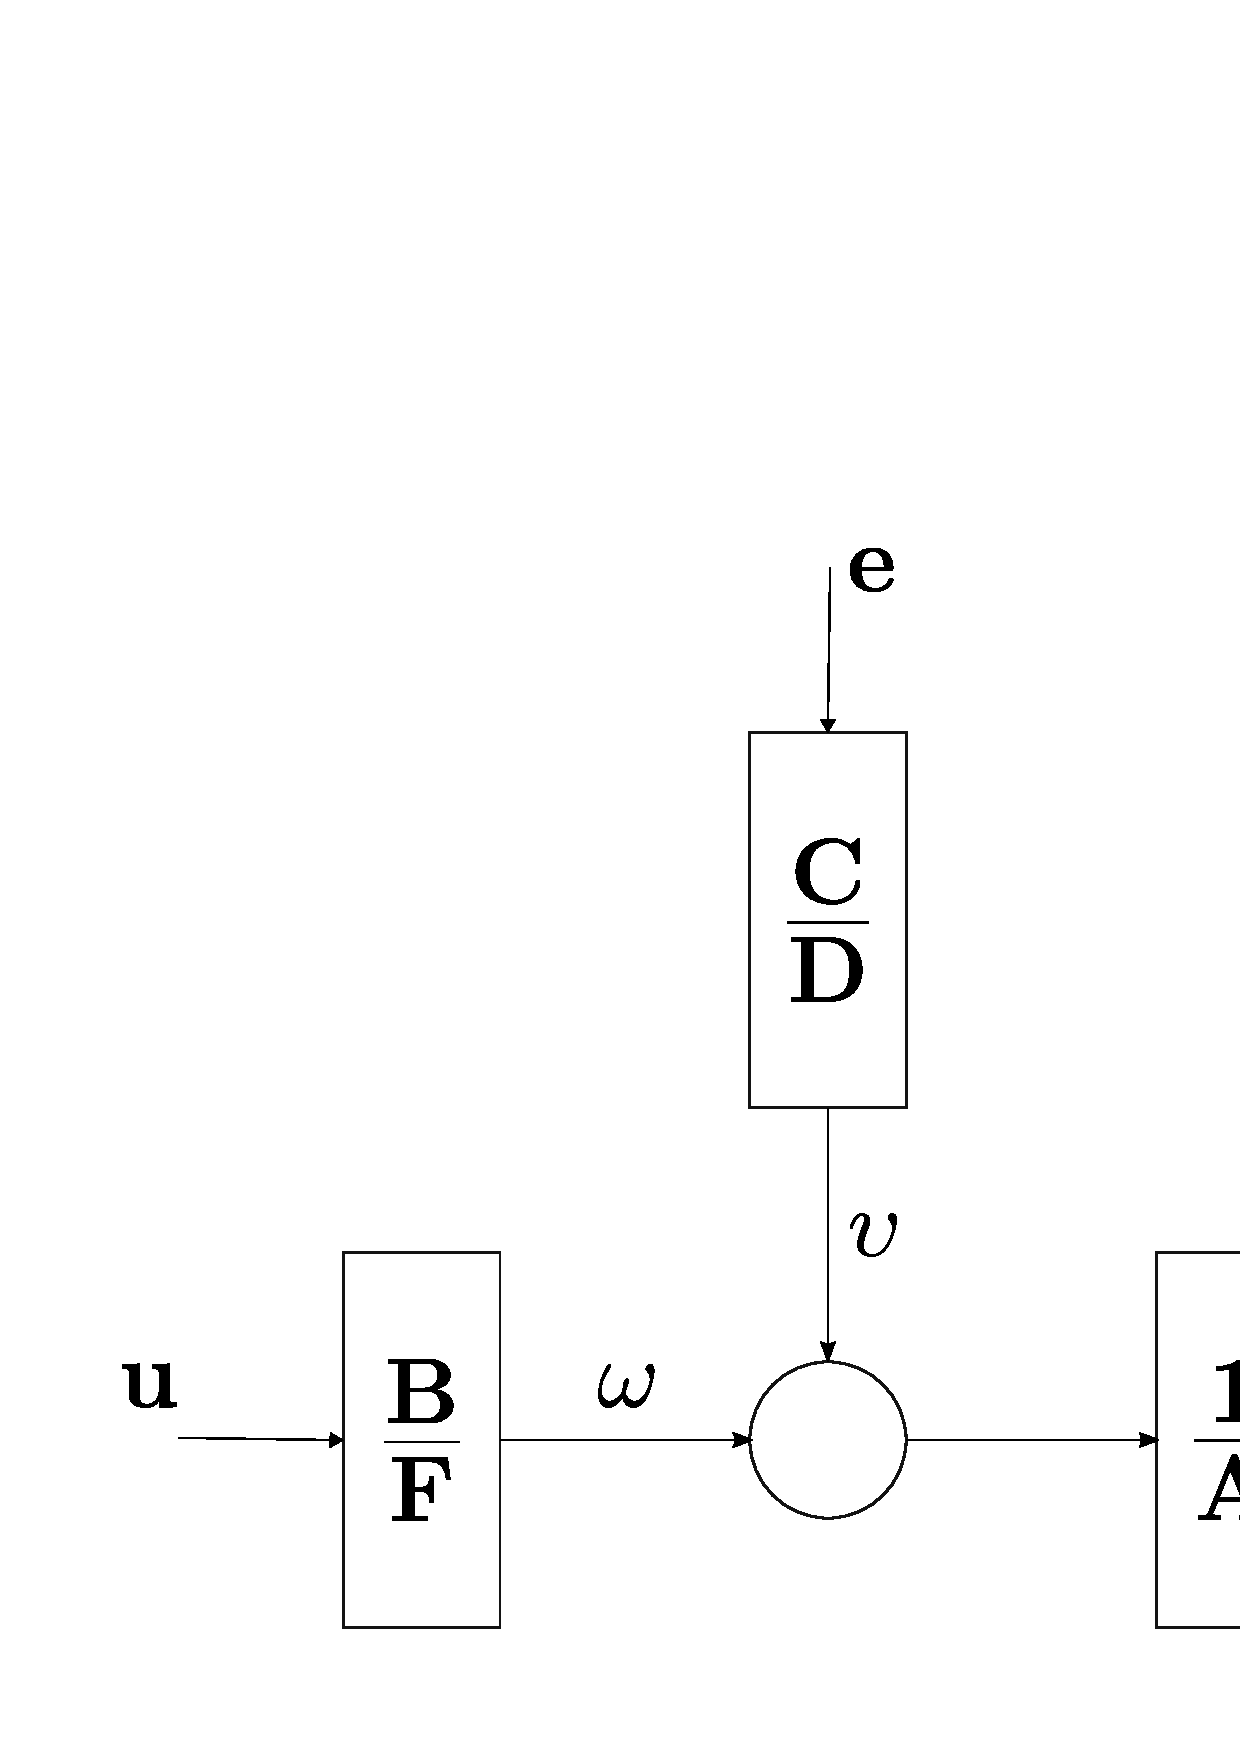
\includegraphics[width=0.5\linewidth]{Inkskape_schemes/linearBBmodel.pdf}
\caption{Scheme of a General Linear Black-box model.}
\label{LinBBsch}
\end{center}
\end{figure}

\subsection{AR model}
\textit{Autoregressive model} or simply AR model does not include relation between system input and output. This method is suitable for signal representation or as a prewhitening filter due to a dependency only on previous outputs and system noise (disturbance). Mathematical form is simple with $\mathbf{B}=0, \mathbf{C}=\mathbf{D}=1$
\begin{equation}
\mathbf{A}(q)y(t)= e(t),
\label{ARForm}
\end{equation} 
$q$ is shift operator, $e(t)$ system noise, $\mathbf{A}(q)= 1 + a_{1}q^{-1} + \dots +a_{k_{a}}q^{-k_{a}}$ is model polynomial in $q^{-1}$ of order $k_{a}$. AR model is depicted via diagram \ref{ARsch}.


\begin{figure} [!ht]
\begin{center}

\includegraphics[width=0.5\linewidth]{Inkskape_schemes/AR.pdf}
\caption{Scheme of a AR Black-box model.}
\label{ARsch}
\end{center}
\end{figure}

\subsection{ARX model}
\textit{Autoregressive with exogenous terms model} or simply ARX model integrate system input - stimulus signal. With special choice of model polynomials $\mathbf{C}=\mathbf{D}=\mathbf{F}=1$ the formula can be written as
\begin{equation}
\mathbf{A}(q)y(t)= \mathbf{B}(q)u(t)+ e(t),
\label{ARXForm}
\end{equation} 
$q$ is shift operator, $e(t)$ system noise, $\mathbf{A}(q)= 1 + a_{1}q^{-1} + \dots +a_{k_{a}}q^{-k_{a}}$, $\mathbf{B}(q)= b_{0} + b_{1}q^{-1} + \dots +b_{k_{b}-1}q^{-k_{b}+1}$ are model polynomials in $q^{-1}$ of orders $k_{a}$ and $k_{b}$ respectively. ARX model is depicted via diagram \ref{ARXsch}.

Form \eqref{ARXForm} can be rewritten 
\begin{equation}
y(t) + a_{1}y(t-1) + \dots +a_{k_{a}} = b_{0}u(t) + b_{1}u(t-1) + \dots + b_{k_{b}-1}u(t-k_{b}+1) +e(t).
\end{equation}
\begin{figure} [!ht]
\begin{center}
\includegraphics[width=0.5\linewidth]{Inkskape_schemes/ARX.pdf}
\caption{Scheme of a ARX Black-box model.}
\label{ARXsch}
\end{center}
\end{figure}

\subsection{ARMAX}
\textit{Autoregressive moving average with exogenous terms model} or simply ARMAX model includes stochastic dynamics. This model can be useful if dominating disturbances enter in process with input. With special choice of model polynomials If model polynomials are chosen specifically  $\mathbf{D}=\mathbf{F}=1$, the formula can be written as
\begin{equation}
\mathbf{A}(q)y(t)= \mathbf{B}(q)u(t)+ \mathbf{C}(q)e(t),
\label{ARMAXForm}
\end{equation} 
$q$ is shift operator, $e(t)$ system noise, $\mathbf{A}(q)= 1 + a_{1}q^{-1} + \dots +a_{k_{a}}q^{-k_{a}}$, $\mathbf{B}(q)= b_{0} + b_{1}q^{-1} + \dots +b_{k_{b}-1}q^{-k_{b}+1}$, $\mathbf{C}(q)= 1 + c_{1}q^{-1} + \dots +c_{k_{c}}q^{-k_{c}}$ are model polynomials in $q^{-1}$ of orders $k_{a}$, $k_{b}$ and $k_{c}$ respectively. ARMAX model is depicted via diagram \ref{ARMAXsch}.

Form \eqref{ARMAXForm} can be rewritten
\begin{align}
y(t) + a_{1}y(t-1) + \dots +a_{k_{a}} &= b_{0}u(t) + b_{1}u(t-1) + \dots + b_{k_{b}-1}u(t-k_{b}+1) \\
&+e(t) +c_{1}e(t-1) + \dots + c_{k_{c}}e(t-k_{c}).
\end{align}

\begin{figure} [!ht]
\begin{center}
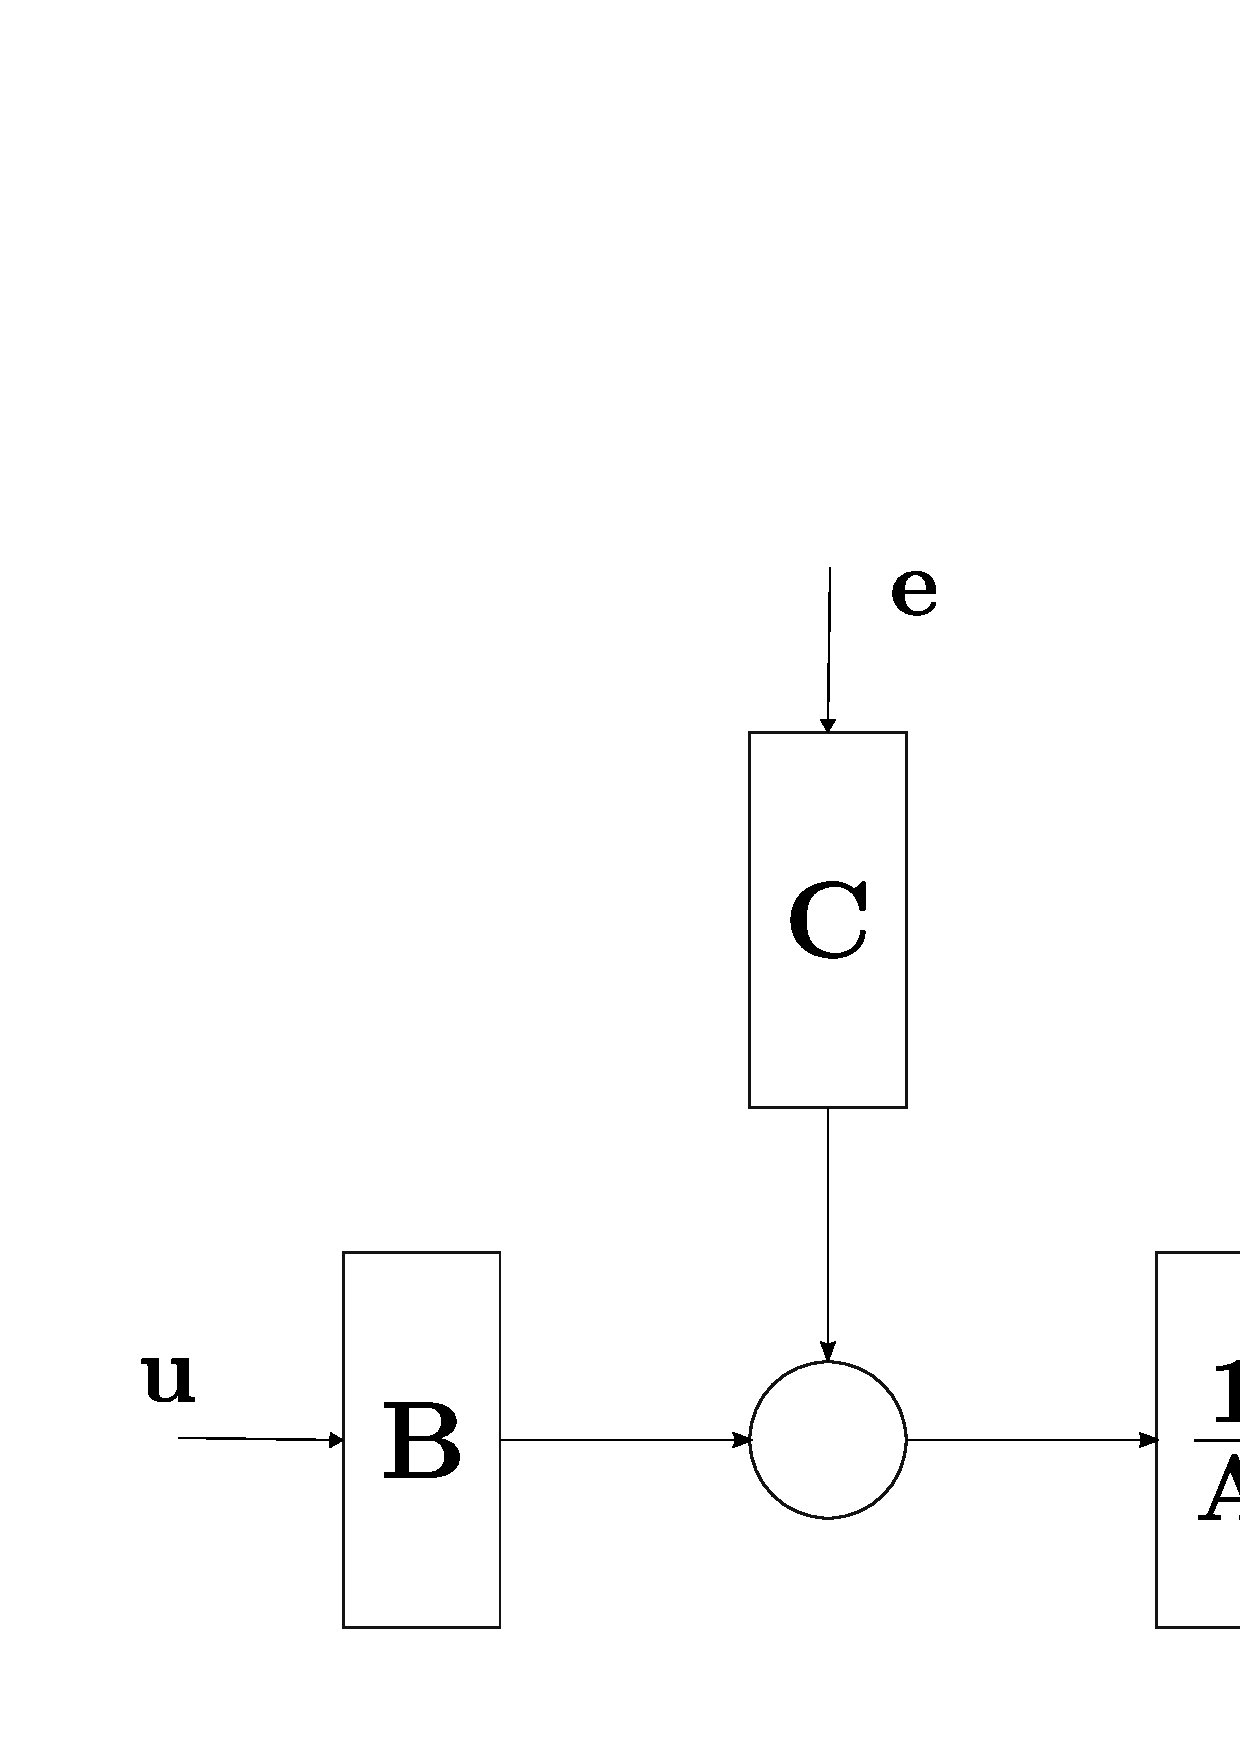
\includegraphics[width=0.5\linewidth]{Inkskape_schemes/ARMAX.pdf}
\caption{Scheme of a ARMAX Black-box model.}
\label{ARMAXsch}
\end{center}
\end{figure}


\subsection{BJ}
\textit{Box-Jenkins model} or shortly BJ model incorporates system dynamicz and system disturbances. Model is useful, when disturbances are connected to measurements (outputs).  BJ model is special case of linear black box model, when $\mathbf{A}=1$. Form is as follows
\begin{equation}
y(t)=\frac{\mathbf{B}(q)}{\mathbf{F}(q)}u(t) + \frac{\mathbf{C}(q)}{\mathbf{D}(q)}e(t),
\label{BJForm}
\end{equation}
$q$ is shift operator, $e(t)$ system noise, $\mathbf{B}(q)= b_{0} + b_{1}q^{-1} + \dots +b_{k_{b}-1}q^{-k_{b}+1}$, $\mathbf{C}(q)= 1 + c_{1}q^{-1} + \dots +c_{k_{c}}q^{-k_{c}}$, $\mathbf{D}(q)= 1 + d_{1}q^{-1} + \dots +d_{k_{d}}q^{-k_{d}}$,$\mathbf{F}(q)= 1 + f_{1}q^{-1} + \dots +f_{k_{f}}q^{-k_{f}}$,  are model polynomials in $q^{-1}$ of orders $k_{b}$, $k_{c}$,$k_{d}$ and $k_{f}$ respectively. BJ model is depicted via diagram \ref{BJsch}, where $\omega,\upsilon$ are auxiliary variables \colorbox{TealBlue}{(ni.com alebo to osdstaniť alebo ešte dohľadať)}.

Form \ref{BJForm} can be rewritten into time domain equations:
\begin{align}
&y(t)=w(t)+v(t),\\
&w(t)+f_{1}w(t-1)+\dots +f_{k_{f}}w(t-k_{f})= b_{0}u(t)+b_{1}u(t-1)+\dots +b_{k_{b}-1}u(t-k_{b}+1)\\
&v(t) + d_{1}v(t-1) + \dots + d_{k_{d}}v(t-k_{d}) = e(t) +c_{1}e(t-1) + \dots + c_{k_{c}}e(t-k_{c}).
\end{align}

\begin{figure} [!ht]
\begin{center}

\includegraphics[width=0.5\linewidth]{Inkskape_schemes/BJ.pdf}
\caption{Scheme of a Box-Jenkins Black-box model.}
\label{BJsch}
\end{center}
\end{figure}

\subsection{OE}
\textit{Output-Error model} or OE model does not use any parameters for simulating disturbances. With a choice $\mathbf{A}=mathbf{C}=mathbf{D}=1$ linear model of this form is OE:
\begin{equation}
y(t)=\frac{\mathbf{B}(q)}{\mathbf{F}(q)}u(t) +e(t),
\label{OEForm}
\end{equation}
$q$ is shift operator, $e(t)$ system noise, $\mathbf{B}(q)= b_{0} + b_{1}q^{-1} + \dots +b_{k_{b}-1}q^{-k_{b}+1}$, ,$\mathbf{F}(q)= 1 + f_{1}q^{-1} + \dots +f_{k_{f}}q^{-k_{f}}$,  are model polynomials in $q^{-1}$ of orders $k_{b}$, and $k_{f}$ respectively. OE model is depicted via diagram \ref{OEsch}

In this case, the model can be also rewritten to the time domain
\begin{align}
&y(t)=w(t)+e(t),\\
&w(t)+f_{1}w(t-1)+\dots +f_{k_{f}}w(t-k_{f})= b_{0}u(t)+b_{1}u(t-1)+\dots +b_{k_{b}-1}u(t-k_{b}+1).
\end{align}

\begin{figure} [!ht]
\begin{center}
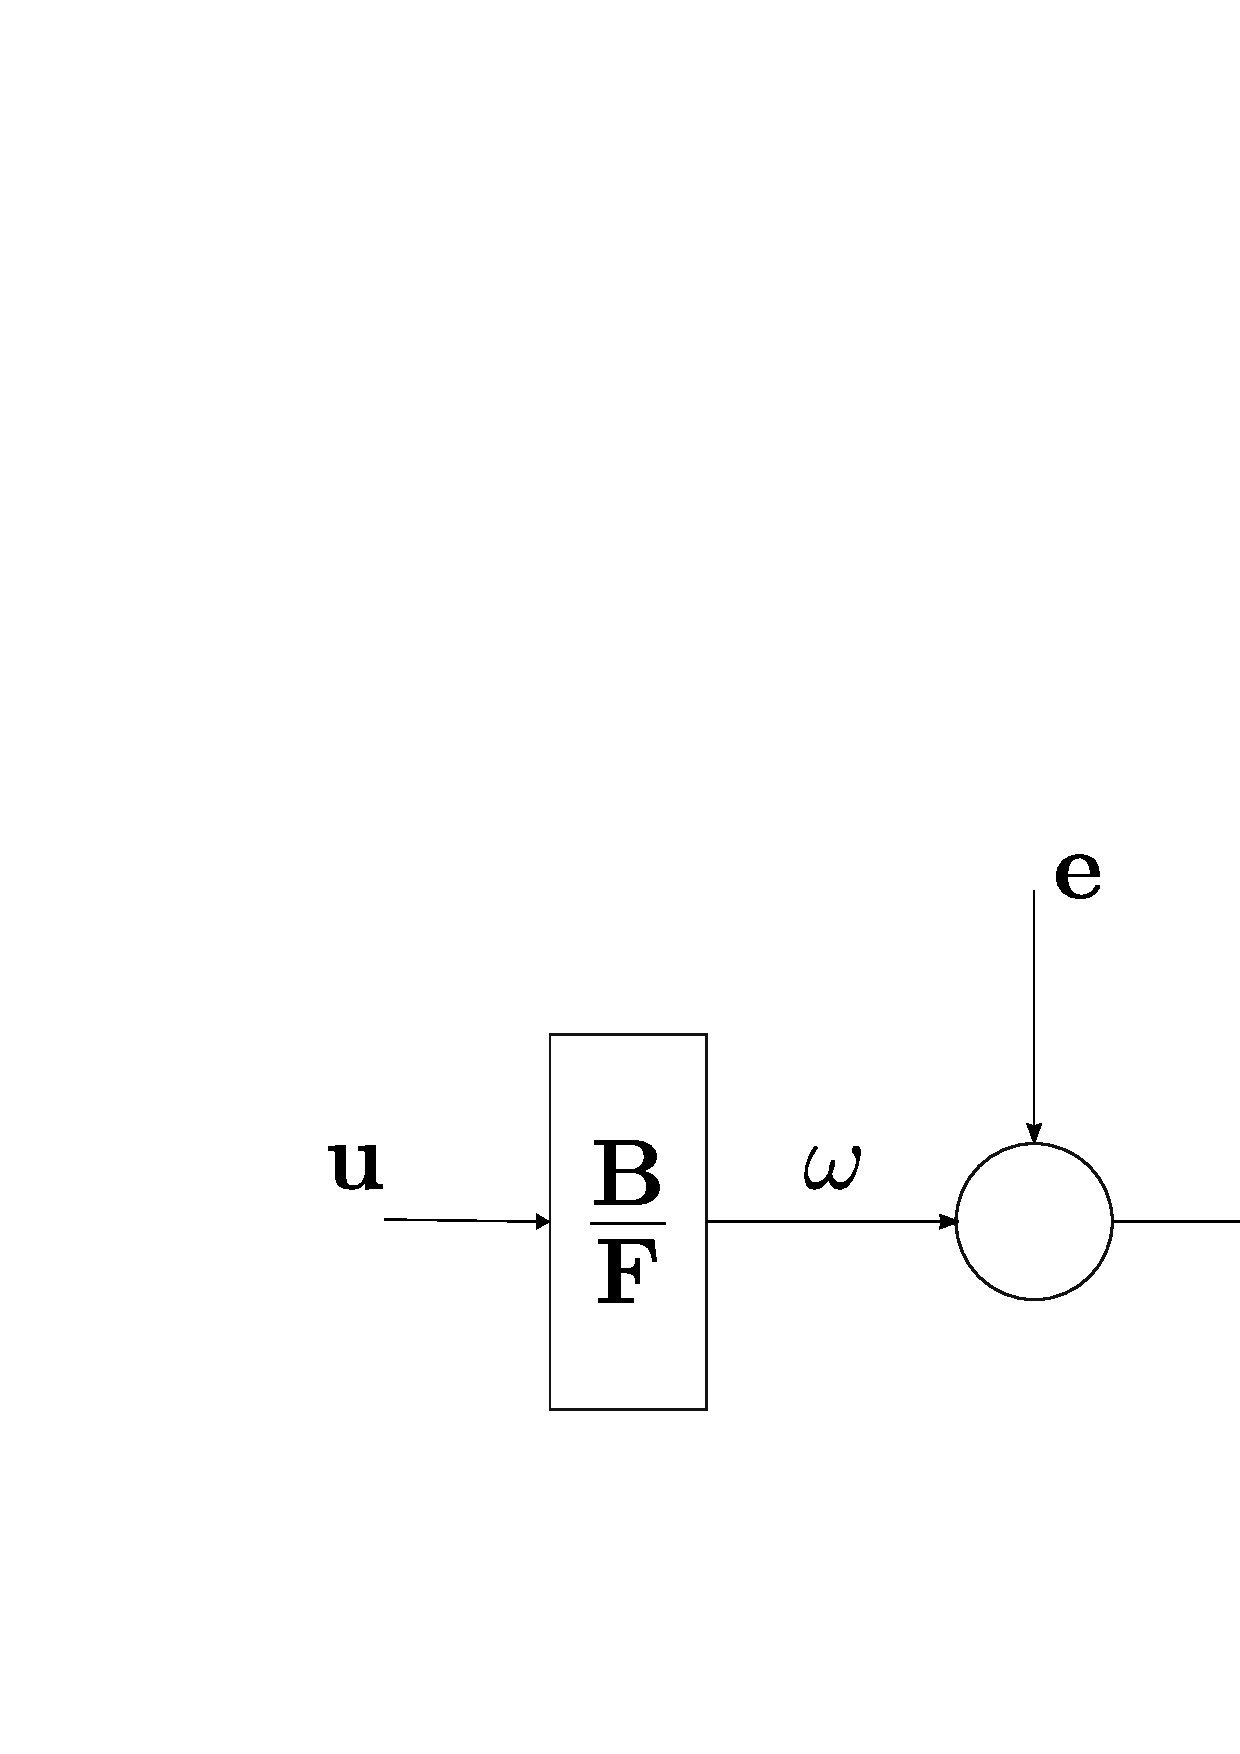
\includegraphics[width=0.5\linewidth]{Inkskape_schemes/OE.pdf}
\caption{Scheme of a Output-Error Black-box model.}
\label{OEsch}
\end{center}
\end{figure}





\section{Non-linear Black-Box Models}

\chapter{Neural Networks}

\chapter{Artificial Data Experiments}

\chapter{Evaluating Models of COMPASS Tokamak}

\section{Electron Problem}

\section{Data}

\section{Models}

\pagestyle{headings}

\chapter*{Conclusion}

\pagestyle{plain}

\addcontentsline{toc}{chapter}{Conclusion}

Text of the conclusion\ldots{}
\begin{thebibliography}{1}
\bibitem{BBmodellingsummary} J. Sjöberg, Q. Zhang, L. Ljung, A. Benveniste, B. Delyon, P. Glorennec, H. Hjalmarsson, A. Juditsky,: \emph{Nonlinear black-box modeling in system identification: a unified overview}. Automatica,Volume 31, Issue 12,1691-1724,ISSN 0005-1098, 1995.
%\bibitem{Allen-Cahn}S. Allen, J. W. Cahn: \emph{A microscopic theory for antiphase boundary motion and its application to antiphase domain coarsening}. Acta Metall., 27:1084-1095, 1979.

%\bibitem{CINECA}G. Ballabio et al.: \emph{High Performance Systems User Guide}. High Performance Systems Department, CINECA, Bologna,2005. \url{www.cineca.it}

%\bibitem{rumpf3}J. Becker, T. Preusser, M. Rumpf: \emph{PDE methods in flow simulation post processing}. Computing and Visualization in Science, 3(3):159-167, 2000.
\end{thebibliography}

\end{document}
